\section{Observation}
\subsection{Clean emotion recognition is governed by structured non-target preference}
\label{sec:clean-emotion-observation}

We first examine whether clean emotion recognition in the model behaves as a hard one-hot decision, or instead as a structured competition over candidate emotions. The latter is clearly supported by our results. Under clean speech, the model does not place all of its confidence on the ground-truth emotion; rather, it consistently preserves non-trivial mass on a small set of emotionally plausible alternatives. Crucially, this residual mass is not random. It follows stable, class-dependent preference patterns, indicating that the model's prediction behavior is governed by a biased geometry within the emotion subspace rather than by generic uncertainty over the whole vocabulary.

\begin{figure*}[!t]
    \centering
    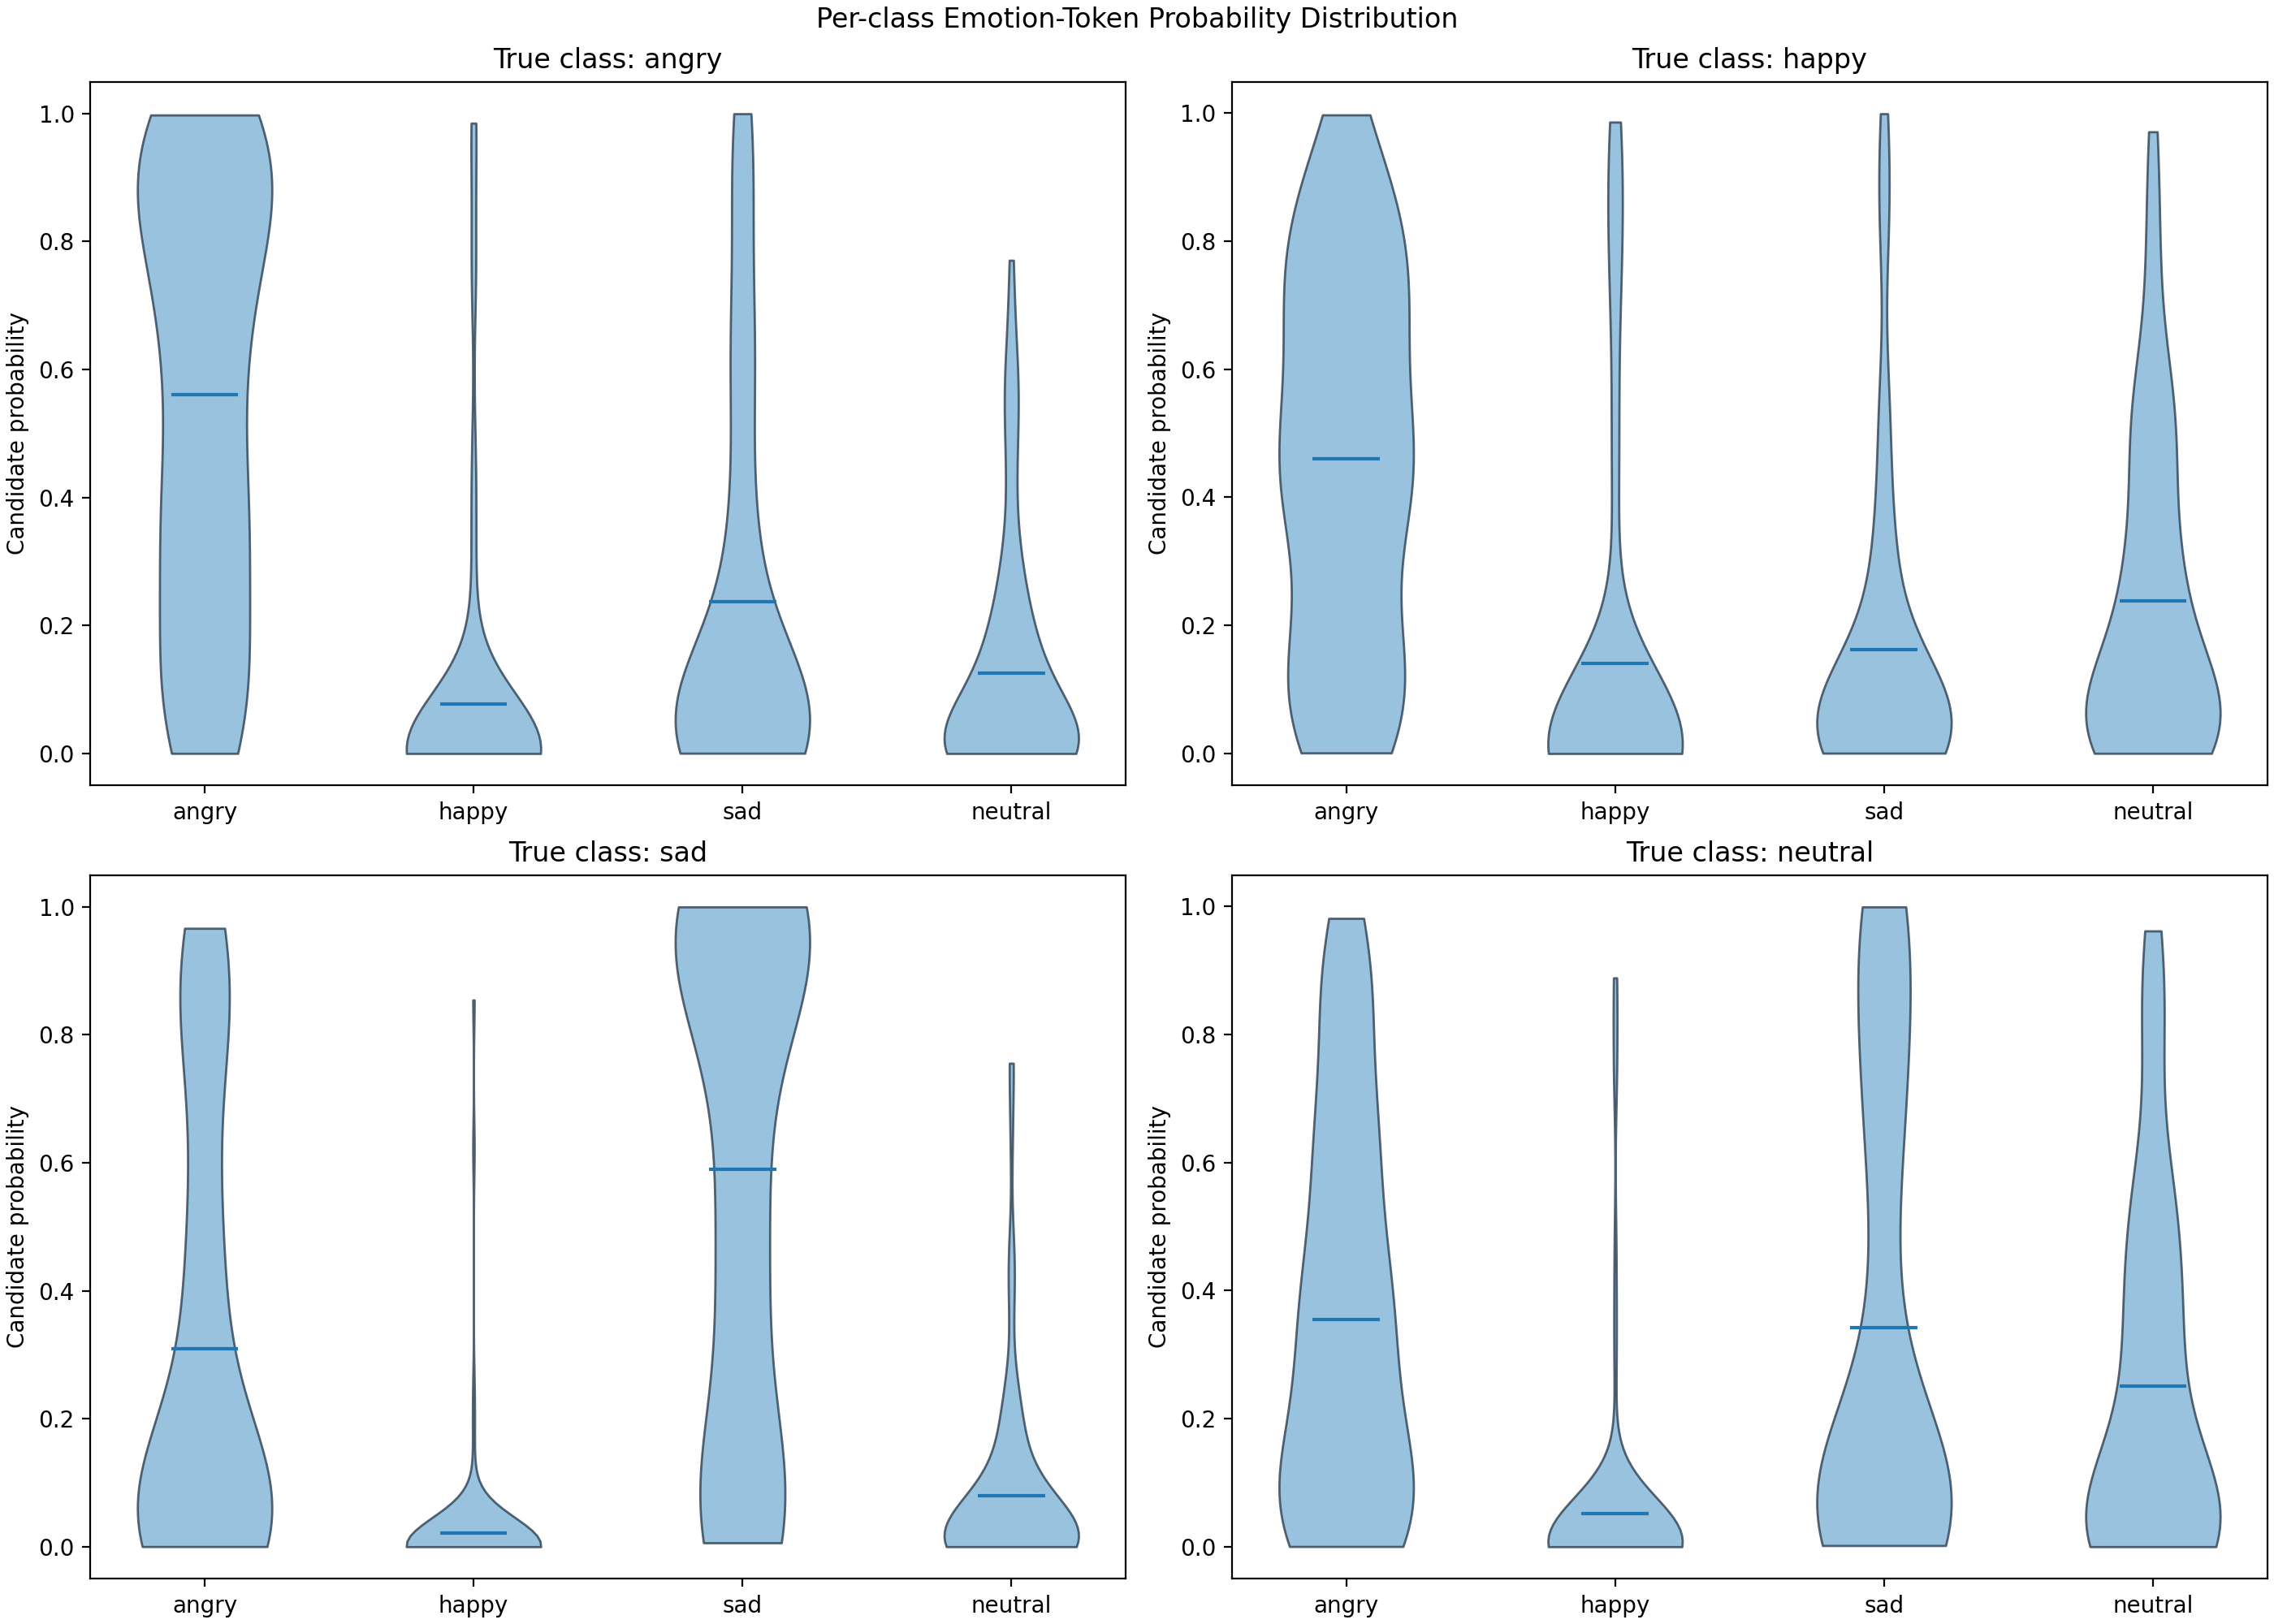
\includegraphics[width=0.82\textwidth]{figure/per_class_emotion_token_probability_distribution.png}
    \caption{
        Per-class candidate probability distributions over \texttt{angry}, \texttt{happy}, \texttt{sad}, and \texttt{neutral} under clean audio-only inputs.
        The posteriors are not one-hot.
        Each true class retains substantial probability mass on specific competing emotions, revealing structured non-target preference rather than uniform uncertainty.
    }
    \label{fig:emotion-prob-structure}
\end{figure*}

Figure~\ref{fig:emotion-prob-structure} shows this phenomenon at the candidate-posterior level. None of the four classes is close to one-hot. \texttt{Angry} and \texttt{sad} show only moderate dominance, with candidate-set accuracies of $0.61$ and $0.63$, while \texttt{happy} and \texttt{neutral} are much less stable, with accuracies of $0.15$ and $0.24$. More importantly, the strongest competitor is not uniform across classes. \texttt{Sad} is the main competitor for true \texttt{angry}, whereas \texttt{angry} is the main competitor for true \texttt{happy}, \texttt{neutral}, and \texttt{sad}. The same asymmetry appears at the prototype level: the closest pair is \texttt{angry}--\texttt{happy} (JS divergence $0.0195$), followed by \texttt{angry}--\texttt{neutral} ($0.0283$), showing that the clean emotion space is already unevenly entangled before any attack is introduced.

\begin{figure*}[!t]
    \centering
    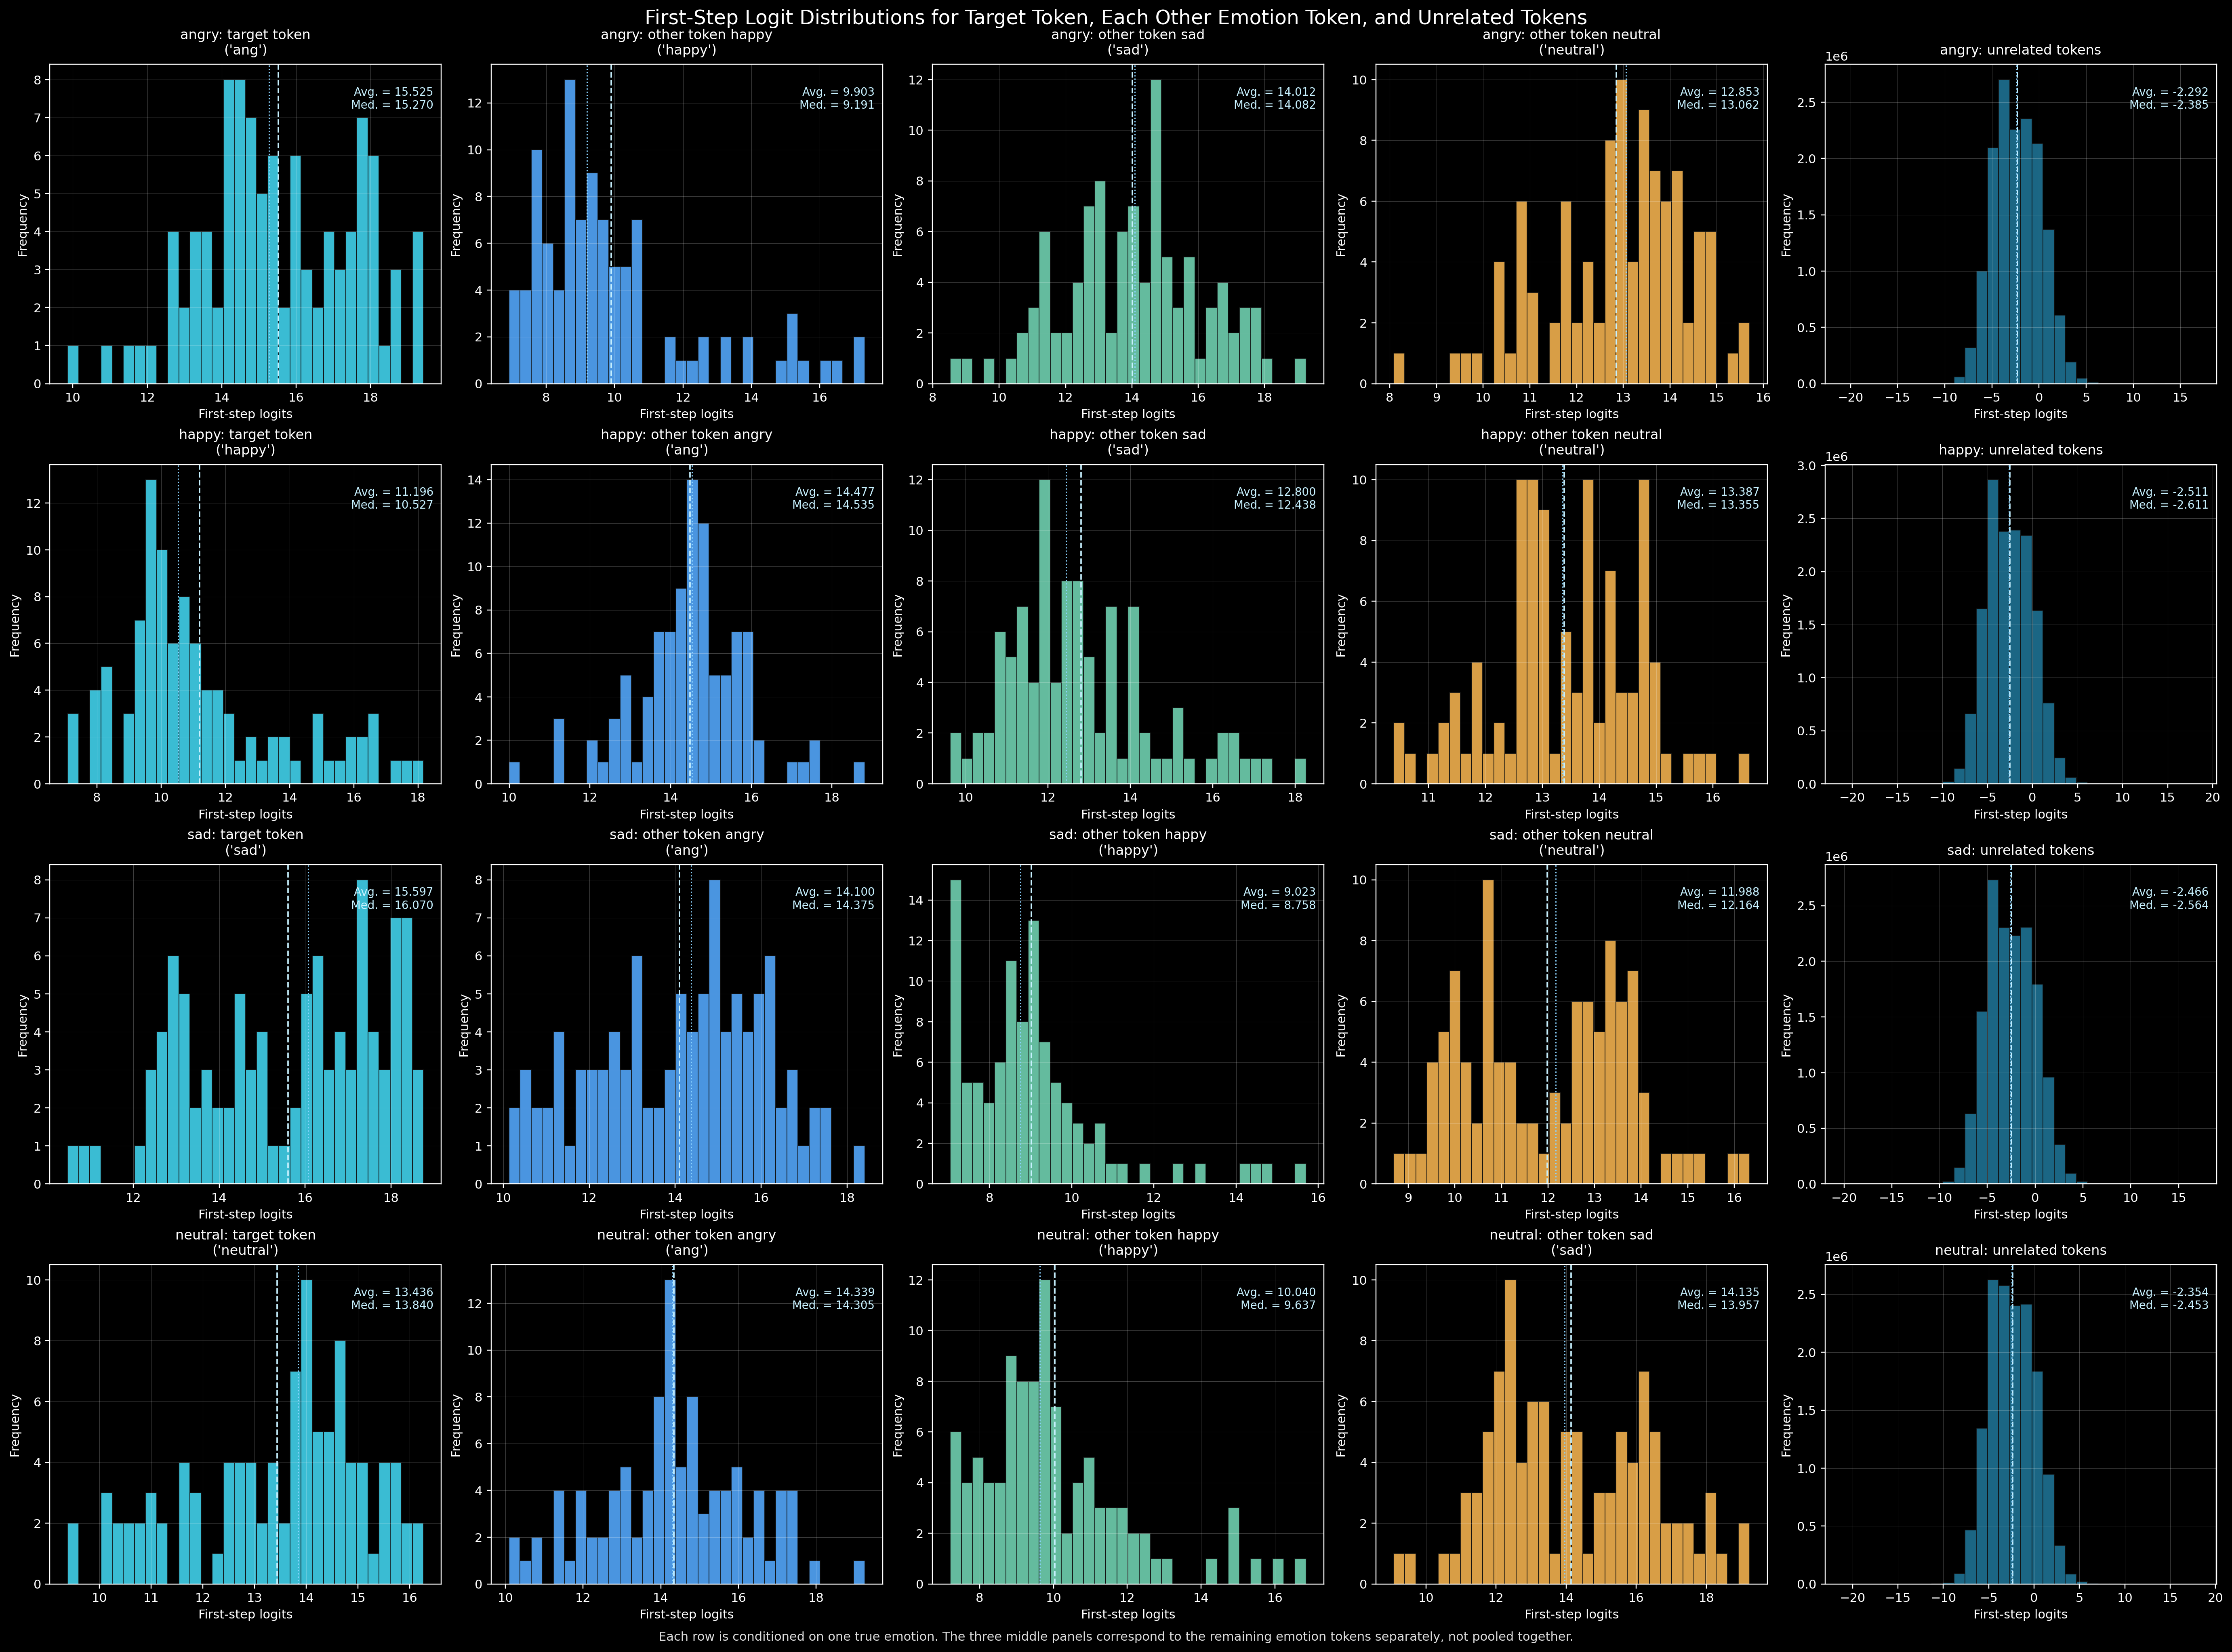
\includegraphics[width=\textwidth]{figure/first_step_target_each_other_unrelated_logit_histograms.png}
    \caption{
        First-step logit distributions for the target emotion token, each non-target emotion token, and unrelated tokens.
        Unrelated tokens remain strongly suppressed across all classes, whereas specific non-target emotion tokens consistently receive elevated logits.
        This shows that the model's uncertainty is concentrated within the emotion subspace, where certain competing emotions are systematically preferred over others.
    }
    \label{fig:first-step-emotion-logits}
\end{figure*}

Figure~\ref{fig:first-step-emotion-logits} provides token-level evidence for the same claim. At the first decoding step, unrelated vocabulary tokens remain strongly suppressed across all four classes, with mean logits around $-2.3$ to $-2.5$, while specific non-target emotion tokens remain highly activated. For example, on true \texttt{happy} samples, the target token \texttt{happy} has mean first-step logit $11.20$, lower than both \texttt{angry} ($14.48$) and \texttt{neutral} ($13.39$); on true \texttt{neutral} samples, the target token \texttt{neutral} has mean logit $13.44$, but both \texttt{angry} ($14.34$) and \texttt{sad} ($14.14$) are higher. This contrast is important: the model is not broadly uncertain over the full vocabulary. Instead, its uncertainty is concentrated inside the emotion token set, where certain alternative emotions are systematically preferred over others. Taken together, the posterior-level and logit-level evidence support a single observation: clean emotion recognition in the model is governed by structured non-target preference. This suggests that downstream objectives should account for inter-emotion geometry, rather than assuming that the clean model already represents emotion as a purely one-hot target.



\subsection{Downstream Impact of Emotion Misperception}
\label{sec:obs_q2}

Beyond the logit-level vulnerability established in Section~\ref{sec:obs_q1}, we ask whether emotion misperception propagates into the model's downstream response behavior. We design an attack-agnostic experiment: for each audio sample, the model (Voxtral-Mini-3B~\cite{voxtral}) receives an \textit{Aligned} prompt (truthful emotion description) and a \textit{Conflict} prompt (false emotion with maximum affective contrast). We evaluate $N = 20$ samples from ESD~\cite{esd} across five emotions. An independent LLM judge (DeepSeek V3~\cite{deepseek}) rates each response on Faithfulness, Empathy, and Relevance (1--5 Likert).

\begin{table}[!t]
\centering
\small
\caption{Response quality degradation under emotion misperception ($\Delta = \text{Aligned} - \text{Conflict}$; higher $=$ greater degradation). 1--5 Likert scale; $n{=}4$ per emotion, $N{=}20$.}
\label{tab:q2_results}
\setlength{\tabcolsep}{8pt}
\begin{tabular}{l@{\hskip 12pt}c@{\hskip 10pt}c@{\hskip 10pt}c}
\toprule
 & \multicolumn{3}{c}{\textbf{Degradation} ($\Delta$)} \\
\cmidrule(lr){2-4}
\textbf{Emotion} & $\Delta_{\text{Faith.}}$ & $\Delta_{\text{Emp.}}$ & $\Delta_{\text{Rel.}}$ \\
\midrule
Angry     & $+0.75$          & $\phantom{+}0.00$ & $\phantom{+}0.00$ \\
Happy     & $+1.75$          & $+3.00$            & $+2.50$            \\
\rowcolor{gray!12}
Sad       & $\phantom{+}0.00$ & $\phantom{+}0.00$ & $\phantom{+}0.00$ \\
Neutral   & $+1.50$          & $+2.00$            & $+0.75$            \\
Surprised & $+2.50$          & $+1.00$            & $+2.00$            \\
\midrule
\textbf{Overall} & $\boldsymbol{+1.30}$ & $\boldsymbol{+1.20}$ & $\boldsymbol{+1.05}$ \\
\bottomrule
\end{tabular}
\end{table}

\textbf{(1) Misperception causes systematic response degradation with pronounced emotion asymmetry.}
As shown in Table~\ref{tab:q2_results}, the Conflict condition degrades all three dimensions (overall: $\Delta_{\text{Faith.}} = +1.30$, $\Delta_{\text{Emp.}} = +1.20$, $\Delta_{\text{Rel.}} = +1.05$), but the effect is highly asymmetric across source emotions. \textit{Happy} is the most vulnerable ($\Delta_{\text{Emp.}} = +3.00$, $\Delta_{\text{Rel.}} = +2.50$), while \textit{sad} is completely robust ($\Delta = 0$ across all dimensions)---the model even explicitly overrides the misleading prompt in some cases, stating ``\textit{They are not angry or frustrated, but rather expressing their grief and pain}.'' This valence-dependent asymmetry, where positive emotions are more susceptible than negative ones, converges with the logit-level fragility of happy identified in Section~\ref{sec:obs_q1}.

\textbf{(2) Misperception induces hallucination in emotionally ambiguous inputs.}
Neutral audio exhibits a distinct failure mode: the model fabricates emotional narratives with no basis in the audio. For a factual statement (``\textit{The package is scheduled to arrive tomorrow afternoon}'') paired with an anger prompt, the model attributes frustration to the speaker, constructs causal explanations, and generates coping strategies---none grounded in the audio content (Faithfulness drops to $1.50/5.00$). This indicates that when audio carries weak emotional signals, the model defaults to the text prompt as its primary emotion source, making emotionally neutral speech---the most common category in real-world deployments---a particularly vulnerable attack surface.

%% ============================================================
%% 2.3  Q3: Insufficiency of Traditional SER Attack Methods
%% ============================================================
\subsection{Insufficiency of Traditional SER Attack Methods}
\label{sec:obs_q3}

We evaluate whether adversarial attack methods developed for Speech Emotion Recognition (SER) transfer to ALLMs. We adapt four representative SER attacks---spanning gradient-based, generator-based, and distortion-based paradigms---to target Voxtral-Mini-3B. All attacks are \textit{untargeted} (strictly easier than targeted flipping). For gradient-based and generator-based methods, we grant full white-box access with a perturbation budget of $\varepsilon = 0.03$ ($L_\infty$), which is $3.75\times$ larger than our ALLM-native attacks ($\varepsilon = 0.008$). The four methods are:

\begin{itemize}\setlength{\itemsep}{2pt}
    \item \textbf{STAA-Net}~\cite{staanet}: A generator-based attack using a Wave-U-Net generator with C\&W untargeted loss~\cite{cw} and sparsity mask. Trained end-to-end with white-box access to Voxtral (200 train / 200 test samples from ESD).
    \item \textbf{PGD}~\cite{pgd}: Projected Gradient Descent on a surrogate SER classifier (wav2vec2-based), achieving 100\% attack success rate on the surrogate, then transferred to Voxtral (525 test samples).
    \item \textbf{Gao et al.}~\cite{gao2022}: Three black-box speech distortions---Vocal Tract Length Normalization (VTLN), McAdams coefficient transformation, and Modulation Spectrum Smoothing (MSS)---originally proposed for SER robustness evaluation (525 test samples each).
    \item \textbf{Ren et al.}~\cite{ren2020}: An atrous CNN generator trained via lifelong learning to attack SER models, then transferred to Voxtral (525 test samples).
\end{itemize}

\begin{figure}[!t]
    \centering
    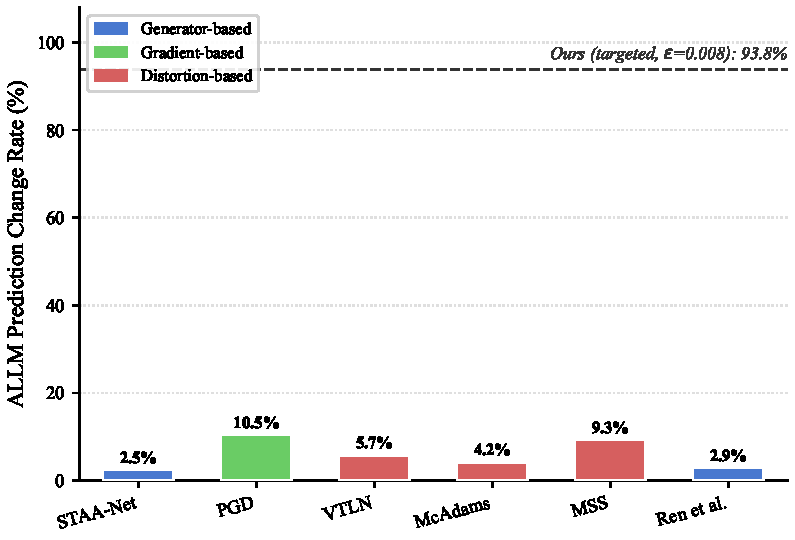
\includegraphics[width=\columnwidth]{figure/q3_ser_transfer.pdf}
    \caption{
        ALLM prediction change rate under six SER adversarial attack methods transferred to Voxtral-Mini-3B.
        All methods alter fewer than 10.5\% of predictions despite using untargeted attacks with $3.75\times$ larger perturbation budgets.
        The dashed line indicates the targeted attack success rate of our ALLM-native method (Section~\ref{sec:methodology}).
    }
    \label{fig:q3_ser_transfer}
\end{figure}

Figure~\ref{fig:q3_ser_transfer} reports the ALLM prediction change rate---the fraction of test samples whose Voxtral emotion prediction differs between clean and adversarial audio. All six methods fail: prediction change rates range from 2.5\% (STAA-Net) to 10.5\% (PGD), with distortion-based methods at 4.2--9.3\% and generator-based methods at 2.5--2.9\%. The failure is particularly striking for PGD, which achieves 100\% attack success on its surrogate SER classifier yet alters only 10.5\% of Voxtral predictions. In contrast, our ALLM-native method achieves 93.8\% \textit{targeted} attack success rate with a $3.75\times$ smaller perturbation budget.

The consistent failure across all paradigms points to a fundamental architectural incompatibility rather than insufficient perturbation magnitude. SER attacks optimize perturbations against standalone classifiers with fixed output spaces, whereas ALLMs route audio through an encoder--adapter--LLM pipeline where emotion judgments emerge via autoregressive generation over a vocabulary of tens of thousands of tokens. The perturbation signal, shaped for a classifier's compact decision boundary, dissipates through the LLM's billion-parameter processing layers before reaching the emotion-relevant decoding steps. This demonstrates that attacking ALLM emotion perception requires methods designed for the autoregressive generation pipeline, motivating the ALLM-native methodology presented in Section~\ref{sec:methodology}.

\subsection{Universal Competitive Structure but Model-Specific Emotion Topology in Audio LLMs}
\label{sec:obs-allm-universal}

We next ask whether the internal emotion mechanism observed above is specific to a single Audio LLM or reflects a broader structural property. To answer this question, we align \texttt{Qwen2-Audio-7B}, \texttt{Voxtral-Mini-3B-2507}, and \texttt{SALMONN-7B} under the same clean probing protocol on a shared 400-sample manifest, and measure both candidate-level emotion competition and layerwise linear separability. This comparison reveals a clear separation between what is \emph{universal} across models and what remains \emph{model-specific}.

% Figure source:
% /home/xuzhenyu/observation_deep_analyze/allm_universality/paper_2_4_final/figures/fig_final_competition_heatmaps.pdf
\begin{figure}[t]
    \centering
    
\includegraphics[width=\linewidth]{figure/fig_final_competition_heatmaps.pdf}
    \caption{\textbf{Cross-model emotion competition fields.} All three Audio LLMs exhibit soft emotion competition rather than hard one-hot classification, but their dominant bias centers differ markedly. Qwen leaks probability mass toward \textit{angry}, Voxtral falls back to \textit{neutral}, and SALMONN is attracted to \textit{happy}. Thus, universality should be stated at the level of \emph{competitive structure}, not at the level of a shared dominant emotion.}
    \label{fig:obs24-final-competition}
\end{figure}

\paragraph{Audio LLMs share a \emph{competitive} internal emotion field, but their dominant bias centers are model-specific.}
Figure~\ref{fig:obs24-final-competition} shows that none of the three models behaves like a hard one-hot emotion classifier. Instead, each source emotion retains substantial probability mass on one or more competitors, forming a stable internal competition field. However, the direction of this leakage is model-dependent. Qwen shows a clear \emph{angry attractor}: for instance, \textit{happy} assigns $0.46$ to \textit{angry} while only $0.14$ remains on \textit{happy}, and \textit{neutral} assigns $0.35$ to \textit{angry}. Voxtral instead exhibits a \emph{neutral fallback}: \textit{angry} assigns $0.53$ to \textit{neutral}, \textit{happy} assigns $0.52$ to \textit{neutral}, and even \textit{neutral} itself remains centered on \textit{neutral} ($0.52$). SALMONN forms a third pattern, namely a \emph{happy attractor}: \textit{angry} assigns $0.32$ to \textit{happy}, \textit{neutral} assigns $0.38$ to \textit{happy}, and \textit{sad} still assigns $0.29$ to \textit{happy}. Therefore, the cross-model invariant is not a shared target emotion, but a shared \emph{competition-based} mechanism with model-specific bias centers.

% Figure source:
% /home/xuzhenyu/observation_deep_analyze/allm_universality/paper_2_4_final/figures/fig_final_midlayer_peaks.pdf
\begin{figure}[t]
    \centering
    
\includegraphics[width=0.78\linewidth]{figure/fig_final_midlayer_peaks.pdf}
    \caption{\textbf{Mid-layer emotion separability peaks before the final layer.} Despite having different bias centers, all three models reach their best probing performance at intermediate layers rather than only at the output layer. This indicates that emotion boundaries emerge in the middle of the LLM stack, creating a natural steering interface for later manipulation.}
    \label{fig:obs24-final-midlayer}
\end{figure}

\paragraph{Emotion separability consistently peaks at intermediate layers, revealing a shared \emph{layered} organization.}
Figure~\ref{fig:obs24-final-midlayer} shows a second cross-model regularity: the best probe layer occurs in the middle of the LLM stack rather than at the final layer. Specifically, the best layer is \texttt{llm\_layer\_06} for Qwen (Macro-F1 $=0.547$), \texttt{llm\_layer\_12} for Voxtral (Macro-F1 $=0.593$), and \texttt{llm\_layer\_06} for SALMONN (Macro-F1 $=0.628$). This pattern is notable because the three models differ substantially in architecture and bias center, yet all of them expose their most separable emotion geometry at intermediate depth. In other words, emotion is not only decided at the final output stage; it already forms a structured representation in the middle layers. This shared layered emergence is precisely what makes internal steering feasible.

\paragraph{These findings point to a \emph{competitor-aware}, \emph{pair-specific}, and \emph{layer-adaptive} attack surface.}
Taken together, the above results imply that later emotion flipping cannot be modeled as generic target-token maximization. Since each model has its own bias center, the easiest source$\rightarrow$target direction depends on the model's own competitor topology. Since the best emotion geometry appears at intermediate layers, internal control should act on representation space rather than only on output logits. And since some pairs align with the model's default bias while others must cross a non-default boundary, controllability is inherently pair-specific. Our pilot results on Qwen and Voxtral are consistent with this interpretation: on nontrivial pairs, \texttt{deep-only} or \texttt{combined} control is more reliable than shallow objectives, whereas bias-aligned pairs are substantially easier to flip. These observations directly motivate the design principles of the next section: the attack objective should be \emph{competitor-aware}, the flip direction should be \emph{pair-specific}, and the control signal should be \emph{layer-adaptive}.
